% Discuss some of the hardware-related work done
% Touch on development of the Gretina card, SBC,
% ORCA, etc.

\chapter{Development of DAQ hardware for \MJ}
\label{app:ORCASoftwareChapter}

	\section{Tundra Universe IID PCI-VME bridge driver}
	\label{sec:TundraUniverse}

This section describes a Linux driver for PCI-VME Tundra Universe II bridge chip.  This
driver is used in Linux kernels newer than 2.6.20 and has been used extensively
with the x86-based lightweight CRUX distribution (\url{http://www.crux.nu}) as
well as Fedora Core (\url{http://fedoraproject.org/}).  The driver is available
at a git repository~\url{http://github.com/mgmarino/VMELinux} as well as in the ORCA subversion
repository~\url{svn://orca.physics.unc.edu/Drivers/SBCDrivers}.  Installation instructions
are given in the code package, so those details are not covered here.

	\lstset{language=csh,
			   backgroundcolor=\color{white},
			   extendedchars=true,
			   basicstyle=\footnotesize\ttfamily,
			   %keywordstyle=\bfseries,
			   showstringspaces=false,
			   showspaces=false,
			   numbers=none,
			   numberstyle=\footnotesize,
			   numbersep=9pt,
			   tabsize=2,
			   breaklines=true,
			   showtabs=false,
			   captionpos=t}
		\subsection{Char driver}

The linux driver package installs a kernel-space driver and installs several devices in 
\lstinline!/dev!, including:
		\begin{lstlisting}
/dev/vme_m[0-7]
/dev/vme_ctl
/dev/vme_dma
		\end{lstlisting}
for the 8~slave image windows of the Universe II chip, a control device, and a DMA transfer device.  The devices can be accessed directly using the Linux \lstinline!ioctl, read, write! 
system calls, though the simpler method for interaction is via the exported API, described later (see Section~\ref{app:DriverAPI}).  The possible ioctl calls are:
	\lstset{language=C++,
			   backgroundcolor=\color{white},
			   extendedchars=true,
			   basicstyle=\footnotesize\ttfamily,
			   %keywordstyle=\bfseries,
			   showstringspaces=false,
			   showspaces=false,
			   numbers=none,
			   numberstyle=\footnotesize,
			   numbersep=9pt,
			   tabsize=4,
			   breaklines=true,
			   showtabs=false,
			   captionpos=t}


		\begin{lstlisting}
UNIVERSE_IOCSET_CTL         // Set CTL of device, but device specific
							// i.e. DMA sets CTL of DMA device, etc.
							// See code for more details 
UNIVERSE_IOCSET_BS			// Set base offset of image 
UNIVERSE_IOCSET_BD			// Set bound (top) of image 
UNIVERSE_IOCSET_VME         // Set VME address offset 
UNIVERSE_IOCSET_IOREMAP     // Set to use ioremap (instead of mmap) 
UNIVERSE_IOCCHECK_BUS_ERROR // Check for an error on the VME bus 

// The following are for the control device ONLY:
UNIVERSE_IOCSET_HW_BYTESWAP // Set the HW byteswap (board specific
							// to Concurrent Technologies boards) 
UNIVERSE_IOCGET_MEM_SIZE    // Get size of PCI memory set aside by driver 
UNIVERSE_IOCGET_BOARD_TYPE  // Return board type 
UNIVERSE_IOCIO_PORT_READ    // Read the IO Port specified by input address 
UNIVERSE_IOCIO_PORT_WRITE   // Write the IO Port at input address 
		\end{lstlisting}
The initialization procedures for each image should be followed:
		\begin{lstlisting}
For a normal image minor, initialize it by (in this order):
	UNIVERSE_IOCSET_CTL: Set control register (address space, data space, etc.)
	UNIVERSE_IOCSET_IOREMAP: set to ioremap pci mem to kernel memory.
	UNIVERSE_IOCSET_BS:	Set base (offset) of window.	The driver will 
        automatically determine where this is within its allowed PCI space.
	UNIVERSE_IOCSET_BD:	Set bound (size) of window.
	UNIVERSE_IOCSET_VME: Use this to set the desired VME address the base
		of the window will point to.

For a DMA minor, initialize it by (in this order):
	UNIVERSE_IOCSET_CTL: Set control register (address space, data space, etc.)
	UNIVERSE_IOCSET_VME: Use this to set the desired VME address from which the 
		DMA will start. 

		\end{lstlisting}
The CTL settings for each image device can be found in the Tundra Universe II manual.  
However, it is much simpler to use the API since this abstracts the behaviour of the
driver.


% Outline the setup, i.e. char devices, dma device, etc.
% ioctl commands

		\subsection{API}
		\label{app:DriverAPI}

The Universe driver API provides a C and \cpp~interface for programming simplicity.
The C interface is simpler, providing a functional-based interface and will be described first.
To use both, add 
		\begin{lstlisting}
#include "universe_api.h"
		\end{lstlisting}
to your code and make sure the API library is in your search path of your compiler, e.g.:
		\begin{lstlisting}
g++ myprog.c -o myprog -L/use/local/universe/lib -luniverse_api
		\end{lstlisting}

			\subsubsection{C API}
The C API is outlined in the following.  If an error occurs during the function, the specified error is set in 
the \lstinline!errno! global.
			\begin{itemize}
			\item\begin{lstlisting}
	extern TUVMEDevice* get_new_device(uint32_t vmeAddress, uint32_t addressModifier, uint32_t dataWidth, uint32_t sizeOfImage = 0);
			\end{lstlisting}
  This function grabs a new device with the given specifications. It will return \lstinline!NULL! if there is any error. 
  An error can be caused if there are no more available devices, or if something is wrong with the input parameters. 
  If \lstinline!sizeOfImage! is 0, then the driver attempts to make the size of the returned device 1/8 of the total pci memory
  space allocated to the Universe II chip. 
  The size of the image specifies how many addresses from the base vmeAddress can be read/written. 
  vmeAddress should be normally 64K aligned (0x10000, with the bottom 16 bits always 0), but there are 
  two devices which have 4K resolution (0x100 aligned).  The driver api will attempt to return one of these
  two devices when the \lstinline!addressModifier! specifies A16, but it is not guaranteed.  
  \lstinline!dataWidth! specifies the width of the data in bytes. 

			\item\begin{lstlisting}
	extern int32_t close_device(TUVMEDevice* device);
			\end{lstlisting}
Closes a device and releases it back into the available pool.  This should be called if a device is no longer being used

			\item\begin{lstlisting}
	extern TUVMEDevice* get_dma_device(uint32_t vmeAddress, uint32_t addressModifier, uint32_t dataWidth);
			\end{lstlisting}
Grabs the dma device and sets up the transfer.  If \lstinline!NULL!, this means that DMA device is busy.
A transfer from the DMA is initiated with the \lstinline!read_device! function.

			\item\begin{lstlisting}
	extern TUVMEDevice* get_ctl_device();
			\end{lstlisting}
Grabs the control device.  If NULL, this means that control device is busy.

			\item\begin{lstlisting}
	extern void set_dma_no_increment(bool noInc = true);
			\end{lstlisting}
This specifies that the dma device should not increment a VME address. This is useful if a dma read
of $x$~bytes is required at one particular address.  It should be called before \lstinline!get_dma_device!.

			\item\begin{lstlisting}
	extern void set_hw_byte_swap(bool doSwap = true);
			\end{lstlisting}
Sets byte swap in the hardware.  This currently only works on the VX 40x/04x Concurrent technologies cpu boards and has undefined behavior for other boards.

			\item\begin{lstlisting}
	extern int32_t read_device(TUVMEDevice*, char* buffer, uint32_t numBytes, uint32_t offset = 0);
			\end{lstlisting}
Reads \lstinline!numBytes! bytes from a device into a buffer at an offset on the device and returns number of bytes read, or less than 0 if error occurs.  

			\item\begin{lstlisting}
	extern int32_t write_device(TUVMEDevice*, char* buffer, uint32_t numBytes, uint32_t offset = 0);
			\end{lstlisting}
Writes \lstinline!numBytes! bytes into a device from a buffer at an offset on the device and returns number of bytes written, or less than 0 if error.

			\item\begin{lstlisting}
	extern uint32_t get_max_size_of_image(void);
			\end{lstlisting}
Returns the maximum size of an image in bytes. 
			\end{itemize}

Some examples of using the functionality are in the following.  Only the `read' variants of the functions are shown, but
the `write' functions behave correspondingly.
			\begin{enumerate}
			\item Grab a device and read from it:
				\begin{lstlisting}
  TUVMEDevice* device = get_new_device(0x0, 0x29, 2, 0x10000); //Map the entire A16 space beginning at 0x0
  char buffer[4];
  if (device == NULL) exit; // Error!
  // read at adress 0x3300 
  if (read_device(device, buffer, 4, 0x3300) < 0 ) { 
    // Error!
    exit;
  }
  // Otherwise we have a successfull read.

  close_device(device);  
  /* This last call is an unnecessary call since the api library handles the closing automatically.  However, if the pool of 8 devices is already empty, this will release a device to be opened/enabled anew via the get_new_device function.  Normally, readout code will set up devices at the beginning of the run so it doesn't need to be done multiple times. */

				\end{lstlisting}
			\item Perform a DMA transfer:
				\begin{lstlisting}
  // Set this if this dma does not auto-increment the address.
  set_dma_no_increment(true); 
  // Set up a DMA transfer, A32, D32 BLT, beginning at address 0x2101000
  TUVMEDevice* device = get_dma_device(0x2101000, 0xB, 4); 
  if (device == NULL) exit; // Error!
  char buffer[4096]; 
  if (read_device(device, buffer, 4096) != 4096) { // DMA transfer 4096 bytes
    //Error!
  }

  /* If the setting on the dma device do not change, it is possible to not call get_dma_device multiple times, but rather hold on to the pointer to the device.  However, the programmer must take care not to change the device settings elsewhere in the code. */
				\end{lstlisting}
  			\item Read/Write from/to the Universe registers

				\begin{lstlisting}
  TUVMEDevice* device = get_ctl_device(); // Grab the ctl device. 
  char buffer[4];
  // the ctl device can only read/write 4 bytes at a time!
  if (read_device(device, buffer, 4, 0x4) < 0 ) { 
    // Error
  } 
				\end{lstlisting}

			\end{enumerate}


			\subsubsection{C++~API}
The C API is actually a wrapper for the \cpp~framework which provides the underlying
API control for the Universe chip.
In the \cpp~framework, each slave image corresponds to an object, \lstinline!TUVMEDevice!.  As well there
exists a singleton (global) which acts as a manager class for all the objects, \lstinline!TUVMEDeviceManager!.
It is suggested to use this singleton class to manage the open and closed image objects, but it is possible
not to.  The singleton class will not `take control' of the images unless the static function 
\lstinline!TUVMEDeviceManager* TUVMEDeviceManager::GetDeviceManager()! is called.  

				\paragraph{\lstinline!class TUVMEDevice!}
A class encapsulating a PCI-VME image.  The interface is defined as:
					\begin{lstlisting}
class TUVMEDevice {

  public:
    TUVMEDevice(uint32_t devNumber);
    virtual ~TUVMEDevice();

    /* Constants for the devices */
    enum ETUVMEDeviceEnum {kNumberOfDevices = 8};
    enum ETUVMEDeviceAddressSpace { kA16 = 0,
                                    kA24 = 1,
                                    kA32 = 2, 
                                    kCRCSR = 3, 
                                    kUser1 = 4, 
                                    kUser2 = 5};
    enum ETUVMEDeviceDataWidth { kD8 = 1,
                                 kD16 = 2,
                                 kD32 = 4,
                                 kD64 = 8};
    enum ETUVMEDeviceMode { kProgram = 0, kData };
    enum ETUVMEDeviceType { kNonPrivileged = 0, kSuper };
    /* End constants */

    /* Set functions to define behaviour of image. */
    inline void SetPCIOffset(uint32_t offset); 
    inline void SetSizeOfImage(uint32_t sizeOfImage);
    inline void SetAddressSpace(ETUVMEDeviceAddressSpace addressSpace); 
    inline void SetDataWidth(ETUVMEDeviceDataWidth dataWidth) 
    inline void SetMode(ETUVMEDeviceMode mode); 
    inline void SetType(ETUVMEDeviceType type);
    inline void SetUseBLTs(bool useBLTs);
    inline void SetAllowPostedWrites(bool allowPostedWrites);
    inline void SetUseIORemap(bool useIORemap);
    void SetVMEAddress(uint32_t vmeAddress); 
    int32_t SetWithAddressModifier(uint32_t addressModifier);
    /* End set functions. */

    /* Introspection functions */
    inline int32_t GetDevNumber() {return fDevNumber;}
    inline uint32_t GetVMEAddress() {return fVMEAddress;}
    inline uint32_t GetSizeOfImage() {return fSizeOfImage;}

    /* Returns a pointer to the image base. */
    inline volatile void* GetMappedAddress(); 

    virtual std::string GetDeviceStringName();

    /* Check if a bus error has occurred */
    int32_t CheckBusError();

    /* Control functions, Open(), should be called,
       then the behaviour set and then Enable called.*/
       Enable will return 0 if successfull. 
    int32_t Open();
    virtual int32_t Enable(); 
    void Close();

    /* Locking functions for thread safety. */
    virtual int32_t LockDevice() { return pthread_mutex_lock( &fLock ); }
    virtual int32_t UnlockDevice() { return pthread_mutex_unlock( &fLock ); }

    /* Read/Write functions */
    int32_t Read(char* buffer, uint32_t numBytes, uint32_t offset = 0);
    int32_t Write(char* buffer, uint32_t numBytes, uint32_t offset = 0);

  protected:
	...
  };

					\end{lstlisting}
All PCI images are memory mapped, meaning that access to the devices occurs by
using a volatile pointer.  Direct access to this pointer is possible using 
\lstinline!volatile void* TUVMEDevice::GetMappedAddress()!.  This pointer
can be used to access the VME bus, but it is up to the user to determine
if an error occurred after access by calling \lstinline!TUVMEDevice::CheckBusError()!.
				\paragraph{\lstinline!class TUVMEControlDevice!}
Defines a control device for the Universe chip and simplifies the calls
available to this device. 
					\begin{lstlisting}
class TUVMEControlDevice: public TUVMEDevice {
  public:
    TUVMEControlDevice();
    virtual ~TUVMEControlDevice();

    /* Constants, cycle speed, board types */
    enum ECycleSpeeds { kNormal  = 0,
                        kFaster  = 1,
                        kFastest = 2 };
    enum EBoardType { 	kUnknown = UNIVERSE_BOARD_TYPE_UNKNOWN,
	              		kCCT     = UNIVERSE_BOARD_TYPE_CCT }; 
    
    /* Access functions */
    int ReadIOPortMemory( uint16_t address );
    int WriteIOPortMemory( uint16_t address, uint8_t value );
    void SetHWByteSwap(bool doByteSwap = true);
    void SetDSNegationSpeed(ECycleSpeeds speed = kNormal);
    void SetDSHighTimeBLTs(ECycleSpeeds speed = kNormal);
    size_t GetPCIMemorySize();
    EBoardType GetBoardType();
    ...
  };
					\end{lstlisting}
				\paragraph{\lstinline!class TUVMEDMADevice!}
Defines the DMA device.  The only additional interface functions are as follows:
					\begin{lstlisting}
class TUVMEDMADevice: public TUVMEDevice {
  public:
    TUVMEDMADevice();
    virtual ~TUVMEDMADevice();
    // Set device to not increment the address during DMA transfer
    void SetNoIncrement(bool noInc = true); 
	...
  };
					\end{lstlisting}
				\paragraph{\lstinline!class TUVMEDeviceManager!}
Defines a manager (singleton) class which is the preferred way to use this API.
The interface of this class is as follows:
					\begin{lstlisting}
class TUVMEDeviceManager {
  public:
    static TUVMEDeviceManager* GetDeviceManager();
    TUVMEDevice* GetDevice(	uint32_t vmeAddress, 
      						uint32_t addressModifier, 
							uint32_t dataWidth, 
							uint32_t sizeOfImage = 0);
    TUVMEDevice* GetControlDevice(); 

    /* DMA read device. */
    TUVMEDevice* GetDMADevice(	uint32_t vmeAddress, 
      							uint32_t addressModifier, 
								uint32_t dataWidth, 
      							bool autoIncrement);
    /* Close the various devices */
    void ReleaseDMADevice(); 
    int32_t CloseDevice(TUVMEDevice* device);

    inline uint32_t GetSizePerImage(); 
    
    void SetUsePostedWrites(bool usePostedWrites = true); 
    
    virtual int32_t LockDevice(); 
    virtual int32_t UnlockDevice(); 
    ...
  };

					\end{lstlisting}
Locking functions are included to enable usage of this object across threads.  Using this
functions is preferable to using a user-defined \lstinline!pthread_lock_t! since 
these functions may be optimized for speed.  

Usage of the singleton class is
similar to usage of the C framework and examples are provided here: 
			\begin{enumerate}
			\item Grab a device and read from it:
				\begin{lstlisting}
  TUVMEDeviceManager* gMgr = TUVMEDeviceManager::GetDeviceManager()
  TUVMEDevice* device = gMgr->GetDevice(0x0, 0x29, 2, 0x10000); //Map the entire A16 space beginning at 0x0
  uint8_t buffer[4];
  if (device == NULL) exit; // Error!
  // read at adress 0x3300 
  if (device->Read(buffer, 4, 0x3300) < 0 ) { 
    // Error!
    exit;
  }
  // Otherwise we have a successfull read.

  gMgr->CloseDevice(device);  
  /* This last call is an unnecessary call since the api library handles the closing automatically.  However, if the pool of 8 devices is already empty, this will release a device to be opened/enabled anew via the get_new_device function.  Normally, readout code will set up devices at the beginning of the run so it doesn't need to be done multiple times. */

				\end{lstlisting}
			\item Perform a DMA transfer:
				\begin{lstlisting}
  TUVMEDeviceManager* gMgr = TUVMEDeviceManager::GetDeviceManager()
  // Set up a DMA transfer, A32, D32 BLT, beginning at address 0x2101000
  TUVMEDevice* device = gMgr->GetDMADevice(0x2101000, 0xB, 4, true); 
  if (device == NULL) exit; // Error!
  char buffer[4096]; 
  if (device->Read(buffer, 4096) != 4096) { // DMA transfer 4096 bytes
    //Error!
  }
  gMgr->ReleaseDMADevice()
				\end{lstlisting}
  			\item Read/Write from/to the Universe registers

				\begin{lstlisting}
  TUVMEDevice* device = gMgr->GetControlDevice(); // Grab the ctl device. 
  char buffer[4];
  // the ctl device can only read/write 4 bytes at a time!
  if (device->Read(buffer, 4, 0x4) < 0 ) { 
    // Error
  } 
				\end{lstlisting}

			\end{enumerate}



% Outline C and C++ interfaces
	%\section{Gretina Mark IV Digitizer}
	%\section{Struck 3302 Digitizer}

	\section{Single-board computers (SBCs)}

	This section briefly describes the framework of the development of
Single-board computers (SBCs) for the \MJ~experiment and related test stands.
This software was built in conjunction with Mark Howe as part of the
ORCA~\cite{Howe08} software package and has been applied to SBCs with VME,
cPCI, and IPE form factors and use with test stands for the
\MJ~experiment~\cite{MJCollaboration}, the KATRIN
experiment~\cite{KatrinCollaboration}, and the SNO+
experiment~\cite{SNO+Collaboration}.  The SBCs in VME crates used the driver
described in the previous section, Section~\ref{sec:TundraUniverse}.  The
software provides two essential run modes: (1) a slow-control mode to set
register settings of cards and (2) a fast readout mode to pull data from cards
resident on the bus. The general software design was to provide an interface to
the ORCA DAQ program, which would allow the behavior of cards to be customized
through register settings, etc.  The fast readout would then be handled by the
SBC to take advantage of the speed of being directly coupled to the bus.  The
SBC would read out the cards on the bus and fill a circular buffer with their
data.  This circular buffer would then be read out asynchronously by the ORCA
program in large chunkcs over a TCP socket.  This type of setup is most useful
given the high bandwidth yet high latency of Gigabit ethernet.  A schematic of
the fast readout is shown in Figure~\ref{fig:SBCReadout}. 

		\begin{figure}
			\centering
			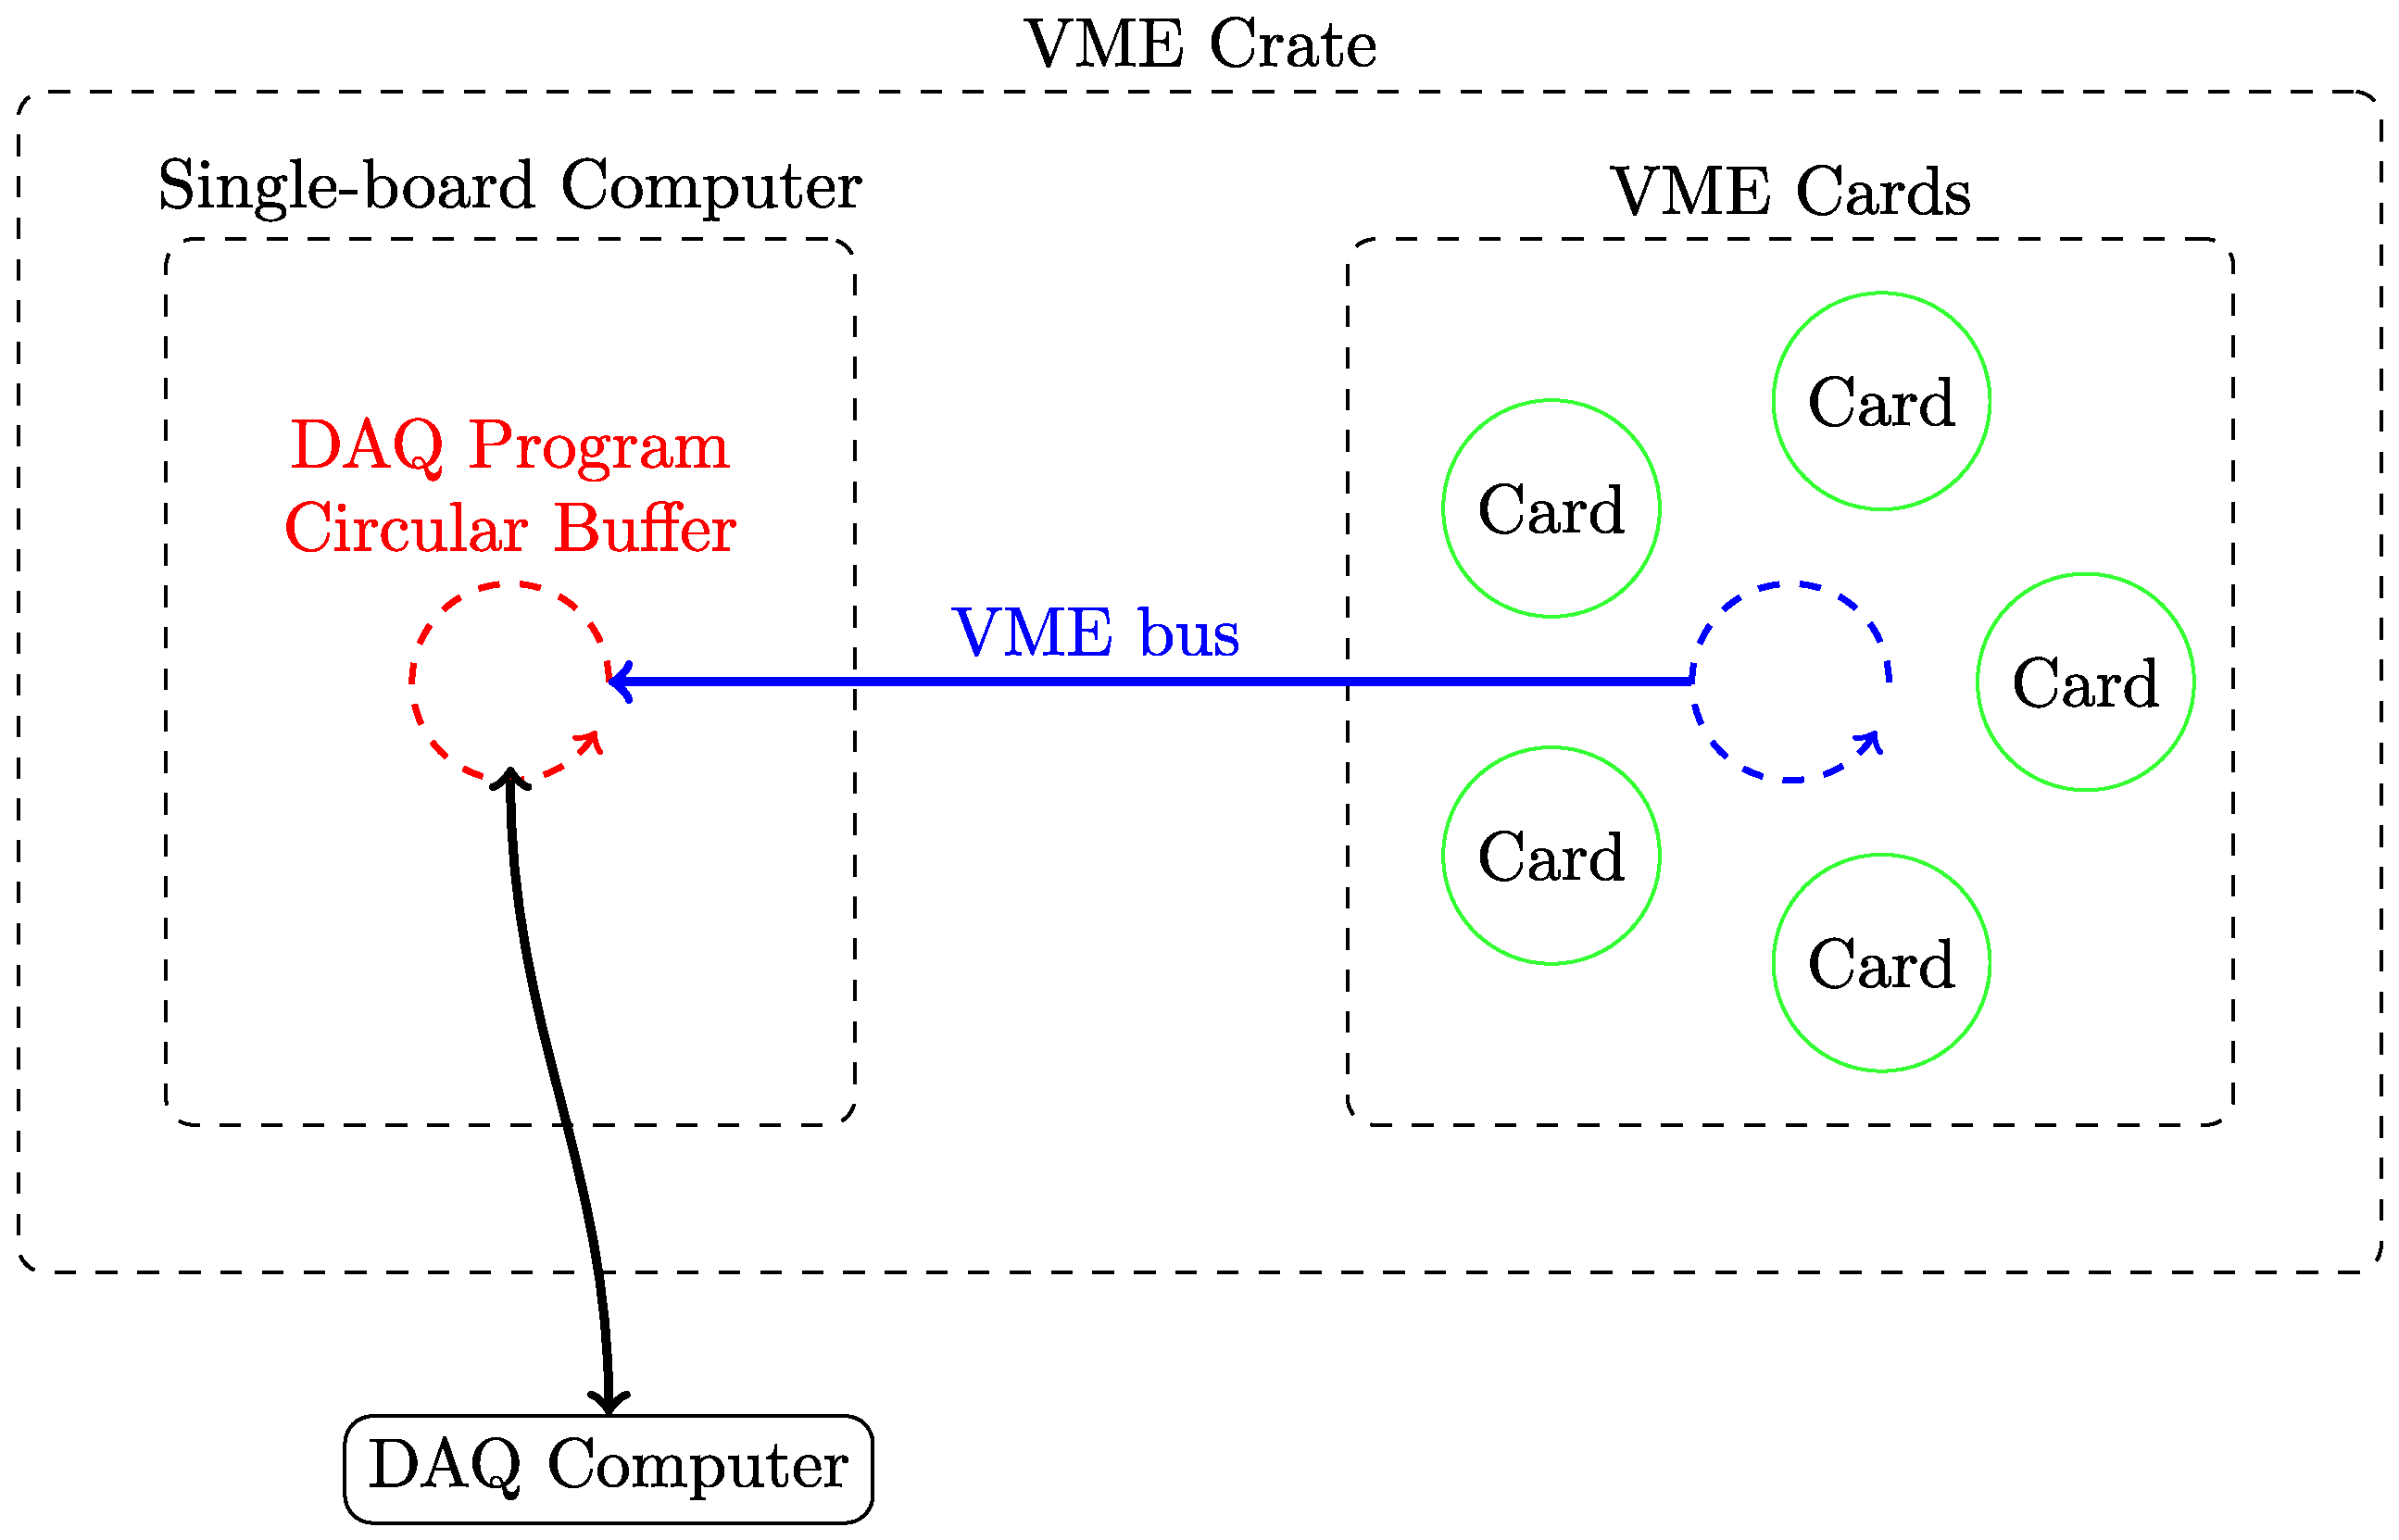
\includegraphics[width=0.8\textwidth]{SBCUsage}
			\caption[A schematic of the SBC data acquisition on a VME bus]
					{A schematic of the SBC data acquisition on a VME bus.  An embedded SBC takes
			         advantage of fast data transfers across the crate bus, filling
			         a circular buffer which is then readout across a TCP socket.
			         The SBC communicates on the VME bus via a PCI-VME `bridge' chip.  
			         The DAQ program on the SBC is a threaded process which takes
			         significant advantage of the dual-core processor onboard.} 
			\label{fig:SBCReadout}
		\end{figure}

		\subsection{SBC card software design}	

\cpp-based software was designed to handle the fast readout of cards on the bus.  A virtual interface was
designed so that a single management program could be created to handle cards of various form factors and designs. 
The virtual base class for this was \lstinline!class ORVCard! described below:
			\begin{lstlisting}

// Struct providing runtime information of the card.
// This is populated and sent from the ORCA DAQ program 
struct SBC_card_info;

// Struct encapsulating Look-at-me (LAM) data 
// to be returned to ORCA 
struct SBC_LAM_Data;

class ORVCard 
{
   public:
       ORVCard(SBC_card_info* ci); 
       virtual ~ORVCard() {} 

      
	   // Overload the following three member functions 
       // to enable readout functionality for a card
       virtual bool Start() { return true; }
       virtual bool Readout(SBC_LAM_Data*) = 0;  
       virtual bool Stop() { return true; }

       // Readout function called by management routine 
       virtual int32_t ReadoutAndGetNextIndex(SBC_LAM_Data*);  

       inline uint32_t GetSlot();
       inline uint32_t GetCrate();
       inline uint32_t GetBaseAddress();
       inline uint32_t GetAddressModifier(); 
       inline uint32_t* GetHardwareMask();
       inline uint32_t* GetDeviceSpecificData();
       inline int32_t GetNextCardIndex();
       inline uint32_t* GetNextTriggerIndex();
       inline uint32_t GetHWTypeID();
       ...
};
			\end{lstlisting}

This interface provides very basic functionality, essentially running the member functions \lstinline!Start! and \lstinline!Stop!
at the start and stop of a run to initialize or shut down a card, and then calling \lstinline!Readout! during a readout cycle.  
The interface could also easily be extended to particular form factors, for example the VME bus, which wraps calls to the Linux
driver API (see Section~\ref{sec:TundraUniverse}).  The following is a truncated example of this:
			\begin{lstlisting}
class TUVMEDevice;
class ORVVmeCard : public ORVCard 
{
   public:
       ORVVmeCard(SBC_card_info* card_info);
       virtual ~ORVVmeCard(); 

    protected:
	/* All the following functions return the bytes written/read,
	   or -1 if an error has occurred. */
	
       // Provide DMA access
       // A corresponding read exists as well 
       static int32_t DMARead(uint32_t vme_address,
                              uint32_t address_modifier,
                              uint32_t data_width,
                              uint8_t* buffer,
                              uint32_t number_of_bytes,
                              bool auto_increment = true);
       ...
       // Provide normal read/write access 
       static int32_t VMERead(uint32_t vme_address,
                              uint32_t address_modifier,
                              uint32_t data_width,
                              uint8_t* buffer,
                              uint32_t number_of_bytes);
       ...
       // Other convenience functions are provided
       // that specify the size of the buffer
       static int32_t VMERead(uint32_t vme_address,
                              uint32_t address_modifier,
                              uint32_t data_width,
                              uint32_t& buffer);
       ...
};
			\end{lstlisting}

		\subsection{SBC management, fast readout design}	

	By designing the code using abstracted functionality, the development of the readout code was simple and is described
fully in the following pythonic pseudocode:
			\lstset{language=Python}
			\begin{lstlisting}
...
allTheCards         # List of cards 
allTheCardsMap = {} # Dictionary to hold the list
# This dictionary is to allow cards to tell the
# management program which card to trigger next
index = 0
for acard in allTheCards:
    allTheCardsMap[index] = acard

# First perform the initialization
for acard in allTheCards:
	acard.Start()

# Now do the readout 
startIndex = 0
while doKeepRunning: # another thread will set this False 
    acard = allTheCardsMap[startIndex]
    startIndex = acard.ReadoutAndGetNextIndex(lamData)
    ... # Handle LAM data

# First perform the shut down 
for acard in allTheCards:
	acard.Stop()

...
			\end{lstlisting}

This simple interface has already been used successfully with multiple different form factors and trigger
types.  As well, the base class has enough functionality to enable complex trigger development.  For example,
a readout of one card might depend on the triggering of another card.  By calling the function \lstinline!ReadoutAndGetNextIndex!, this enables the code in the card class to control the flow of the readout loop. This simple and robust design
has simplified debugging, streamlining both the hardware and development process.
%The management code was written
%in C, so the calling of the \cpp~code was wrapped using the following set of code:
%  			\begin{lstlisting}
%...
%// Header file 
%extern "C" {
%class ORVCard;
%#else
%struct ORVCard;
%#endif
%
%// Returns number of cards loaded.
%int32_t load_card(SBC_card_info* card_info, int32_t index);
%int32_t start_card(int32_t index);
%int32_t readout_card(int32_t index, SBC_LAM_Data* lam_data);
%int32_t stop_card(int32_t index);
%int32_t remove_card(int32_t index);
%// Returns the ORVCard* at the index
%// NULL if cannot find
%#ifndef __cplusplus
%struct
%#endif
%ORVCard* peek_at_card(int32_t index);
%
%#ifdef __cplusplus
%}
%#endif
%    		\end{lstlisting}
%    		\begin{lstlisting}
%// Source file, wrapping C++ calls
%#include "readout_code.h"
%#include <map>
%std::map<int32_t, ORVCard*> gSetOfCards;
%std::map<int32_t, ORVCard*>::iterator gCardIterator;
%
%// Following file pulls in the necessary readout initialization for this code
%#include "HW_Specific.icc"
%
%// Returns number of cards loaded.
%int32_t readout_card(int32_t index, SBC_LAM_Data* lam_data)
%{
%  gCardIterator = gSetOfCards.find(index); 
%  if (gCardIterator == gSetOfCards.end()) return -1;
%  return (gCardIterator->second->ReadoutAndGetNextIndex(lam_data));
%  
%}
%
%// Returns number of cards started.
%int32_t start_card(int32_t index)
%{
%  gCardIterator = gSetOfCards.find(index); 
%  if (gCardIterator == gSetOfCards.end()) return 0;
%  gCardIterator->second->Start();
%  return 1;
%}
%
%// Returns number of cards stopped.
%int32_t stop_card(int32_t index)
%{
%  gCardIterator = gSetOfCards.find(index); 
%  if (gCardIterator == gSetOfCards.end()) return 0;
%  gCardIterator->second->Stop();
%  return 1;
%}
%
%// Returns number of cards removed.
%int32_t remove_card(int32_t index)
%{
%  gCardIterator = gSetOfCards.find(index); 
%  if (gCardIterator == gSetOfCards.end()) return 0;
%  delete gCardIterator->second;
%  gSetOfCards.erase(gCardIterator);
%  return 1;
%}
%
%ORVCard* peek_at_card(int32_t index)
%{
%  gCardIterator = gSetOfCards.find(index); 
%  if (gCardIterator == gSetOfCards.end()) return NULL;
%  return (gCardIterator->second);
%}
%    		\end{lstlisting}
%
%The management code was then as simple as:
%    		\begin{lstlisting}
%void initializeHWRun(SBC_crate_config* config)
%{
%    int32_t index = 0;
%    while(index<config->total_cards){
%        if (load_card(&config->card_info[index], index) != 1) {
%            // Error
%        }
%        index++;
%    }
%}
%void startHWRun (SBC_crate_config* config)
%{    
%    int32_t index = 0;
%    while(index<config->total_cards){
%        if (start_card(index) != 1) {
%            // Error
%        }
%        index++;
%    }
%}
%
%int32_t readHW(SBC_crate_config* config,int32_t index, SBC_LAM_Data* lamData)
%{
%    if(index<config->total_cards && index>=0) {
%        return readout_card(index, lamData);
%    }
%    return -1;
%}
%
%
%void stopHWRun (SBC_crate_config* config)
%{
%    int32_t index = 0;
%    while(index<config->total_cards){
%        if (stop_card(index) != 1) {
%            // Error
%        }
%        index++;
%    }
%}
%
%void cleanupHWRun (SBC_crate_config* config)
%{
%    int32_t index = 0;
%    while(index<config->total_cards){
%        if (remove_card(index) != 1) {
%            // Error
%        }
%        index++;
%    }
%}
%
%
%    		\end{lstlisting}
%where \lstinline!readHW! could be called in a tightly-looped thread for fast readout.
